\documentclass[aspectratio=169]{beamer}
\usepackage{booktabs}
\usepackage{svg}
\usepackage{listings}
\usepackage{fontawesome}
\usepackage{xcolor}
\usepackage{bookmark}
\usepackage{longtable}
\usepackage{amsmath}
\usepackage{minted}
\usepackage{fontawesome}
\newenvironment{rcases}
  {\left.\begin{aligned}}
  {\end{aligned}\right\rbrace}
\definecolor{lightgray}{rgb}{0.97, 0.97, 0.97}
\usepackage[style=numeric,citestyle=ieee
,backend=bibtex]{biblatex}

    \newcommand{\red}[1]{{\color{red}{#1}}}
    \newcommand{\blue}[1]{{\color{blue}{#1}}}

    \lstset{
        basicstyle=\ttfamily,
        numbers=left,
        keywordstyle=\color[rgb]{0.13,0.29,0.53}\bfseries,
        stringstyle=\color[rgb]{0.31,0.60,0.02},
        commentstyle=\color[rgb]{0.56,0.35,0.01}\itshape,
        numberstyle=\footnotesize,
        stepnumber=1,
        numbersep=5pt,
        backgroundcolor=\color[RGB]{248,248,248},
        showspaces=false,
        showstringspaces=false,
        showtabs=false,
        tabsize=2,
        captionpos=b,
        breaklines=true,
        breakatwhitespace=true,
        breakautoindent=true,
        escapeinside={\%*}{*)},
        linewidth=\textwidth,
        basewidth=0.5em,
    }

% \newcommand{\red}[1]{{\color{red}{#1}}}
\newcommand{\redline}[1]{{\color{red}{\ul{#1}}}}
\newcommand{\redlineit}[1]{{\color{red}{\ul{\textit{#1}}}}}
\newcommand{\redit}[1]{{\color{red}{\textit{#1}}}}
\newcommand{\redbf}[1]{{\color{red}{\textbf{#1}}}}

\newcommand{\underit}[1]{\ul{\textit{#1}}}

\newcommand{\blueit}[1]{{\color{blue}{\textit{#1}}}}
% \newcommand{\blue}[1]{{\color{blue}{#1}}}
\newcommand{\blueline}[1]{{\color{blue}{\ul{#1}}}}

\usecolortheme{seagull}
\setbeamertemplate{sidebar right}{}
\setbeamertemplate{footline}{%
	\hfill\usebeamertemplate***{navigation symbols}
    \hspace{1cm}\insertframenumber{}/\inserttotalframenumber}
\setbeamertemplate{section in toc}[sections numbered]
    
\title{The Big-O Problem for Labelled Markov Chains and Weighted Automata\footfullcite{chistikov2020big}}
\date{\today}
\addbibresource{ref.bib}
\setcounter{section}{-1}
\begin{document}
\begin{frame}
    \titlepage
\end{frame}

\begin{frame}{Findings}
    \begin{enumerate}
        \item The big-O problem for non-negative Weighted Automata (WA) and  Labelled Markov Chains (LMCs) turns out to be \red{undecidable in general}.
        \item For \textbf{unambiguous} automata, i.e., where every word has at most one accepting path, the big-O problem becomes \blue{decidable} and can be solved in \blue{polynomial time}.
        \item In the \textbf{unary} case, i.e., if the input alphabet $\Sigma$ is a singleton, the big-O problem is
        also \blue{decidable} and, in fact, \textbf{coNP}-complete.
        \item In a more general \textbf{bounded} case, if the languages of all words $w$ associated with non-zero weight are included in  $w_1^*w_2^*\cdots w_m^*$ for some finite words  $w_1,w_2,\cdots, w_m \in \Sigma^*$, the big-O problem is \blue{decidable} \textit{subject to} Schanuel’s conjecture.
    \end{enumerate}
\end{frame}

\begin{frame}{Overview}
    \tableofcontents
\end{frame}

\section{Background}
\begin{frame}{Weighted Automata}
    \begin{block}{$\langle Q, \Sigma,M,F\rangle$: A Weighted Automaton $\cal W$}
        Over a semi-ring $(\mathbb{Q}, +, \times)$
        \begin{description}
            \item[$Q$] a finite set of states
            \item[$\Sigma$] a finite alphabet
            \item[$M$] $\Sigma \to \mathbb{Q}^{Q \times Q}$, a transition weighting function
            \item[$F$] $\subseteq Q$ a set of final states
        \end{description}
        Non-negative Weighted automata:  $\forall a \in \Sigma, \forall q,q^\prime \in Q \to M(a)(q,q^\prime) \ge 0 $
    \end{block}

    For an input $w \in \Sigma^*$ and a state $s \in Q$,define a function $f_s: \Sigma^\prime \to \mathbb{R}$

    $$f_s(w) = \sum_{t \in F} (M(a_1) \times M(a_2) \times \cdots \times M(a_n))_{s,t} \quad \text{for} \quad  a_1 a_2 \ldots a_n \in w$$
    stands for the weight of $w$ from state $s$
\end{frame}

\begin{frame}{Positive Weight Word Set}
    A set of all $w$ with \red{positive} weight from state $s$
    $$\begin{aligned}
            {\cal L}_s({\cal W}) & = \{w | w \in \Sigma^* \land f_s(w) > 0\}        \\
                                 & \to \text{the language of } {\cal N}_s({\cal W})
        \end{aligned}$$

    \begin{block}{}

        ${\cal N}_s({\cal W})$: the
        \textit{non-deterministic finite automaton} (NFA) formed from the \blue{same} set of states ($Q$ and $F$) as $\cal W$, start state $s$, and transitions $q \xrightarrow{a} q^\prime$ whenever $M(a)(q,q^\prime) > 0$
    \end{block}
\end{frame}

\begin{frame}{Problem Definition}
    \begin{block}{What is big-O?}
        Given $s,s^\prime \in Q$:
        $$
            \begin{aligned} \exists C>0, \forall w \in \Sigma^*, & f_s(w) \le C \cdot f_{s^\prime}(w)  \\
                                                     & \Downarrow                          \\
                s                                    & \text{ \red{is big-O of} } s^\prime
            \end{aligned}
        $$
    \end{block}

    Big-O and Big-$\Theta$ problems can be reduced to each other:
    $$
        \begin{rcases}
            s \text{ is big-O of } s^\prime \\
            s^\prime \text{ is big-O of } s
        \end{rcases}
        \Leftrightarrow s \text{ is big-}\Theta \text{ of } s^\prime
    $$
\end{frame}

\begin{frame}{Labelled Markov Chain (LMC)}
    A special class of weighted automata
    \begin{definition}
        A non-negative weighted automaton $\langle Q, \Sigma,M,F\rangle$ that: $\forall q \in Q  \backslash F$
        \begin{itemize}
            \item $\sum_{q^\prime \in Q} {\sum_{a \in \Sigma}{M(a)(q,q^\prime)}} = 1$
            \item $M(a)(q,q^\prime) = 0$
        \end{itemize}
    \end{definition}
    \begin{itemize}
        \item Final states have no outgoing transitions
        \item $f_s(E) = \sum_{w \in E} f_s(w) \le 1$ for a $E \subseteq \Sigma^*$
        \item The probability (weight) of a transition $q \to q^\prime$ is fixed \textit{independently} of the past sequence of states visited by the machine
    \end{itemize}
\end{frame}

\begin{frame}{Measurements}
    \begin{block}{}
    For two states $s$ and $s^\prime$, define the (asymmetric) ratio variation function as:
    $$r(s,s^\prime) = \sup_{E \subseteq \Sigma^*} (f_s(E) / f_{s^\prime}(E))$$
\end{block}
    The big-O problem $\implies$ whether $r(s,s^\prime) < \infty$
    

\begin{block}{The ratio distance (symmetric)}

    $$rd(s,s^\prime)= \max(r(s,s^\prime),r(s^\prime,s))$$
\end{block}

    A system $\cal M$ is $\epsilon$-differentially private if
    $$\forall s,s^\prime \in Q, \forall E \in \Sigma^*, \quad f_s(E) \le e^\epsilon f_{s^\prime}(e)$$
    $r$ captures the level of differential privacy between $s$ and $s^\prime$
\end{frame}

\section{Undecidability Results in General}
\begin{frame}{Big-O, Threshold and Approximation Problems are \red{Undecidable}}
    \begin{itemize}
        \item The big-O problem is \red{undecidable}, even for LMCs
        \item Each variation of the problem
        \begin{itemize}
            \item asymmetric/symmetric ($r$ vs. $rd$)
            \item non-strict/strict
            ($\le$ vs. $<$)
        \end{itemize}
        is \red{undecidable}, even under the promise of \textbf{boundedness}
        \item All variants of the \blue{approximation} tasks are \red{unsolvable}, even under the promise of boundedness.
        \begin{itemize}
            \item asymmetric/symmetric ($r$ vs. $rd$)
        \end{itemize}
        
        \blue{Approximation}: Find a $x$ for a given constant $\gamma$ that
        \begin{columns}
            \begin{column}{.4\textwidth}
                \begin{block}{Addictive}
                    $|r(s,s^\prime) - x|\le \gamma$ 
                \end{block}
            \end{column}
            \begin{column}{.1\textwidth}
                vs.
            \end{column}
            \begin{column}{.4\textwidth}
                \begin{block}{Multiplicative}
                    $1-\gamma \le \frac{x}{r(s,s^\prime)}\le 1+ \gamma$ 
                \end{block}
            \end{column}
        \end{columns}
    \end{itemize}
\end{frame}

\begin{frame}{The LC condition: A simple \red{necessary} (but \textcolor{gray}{insufficient}) condition of big-O}
    \framesubtitle{language containment condition}
    If $s$ is big-O of $s^\prime$, then
    \begin{block}{LC condition}
        If for all words $w$ with $f_s(w) > 0$ we also have $f_{s^\prime} (w)>0$. Equivalently,
        $${\cal L}_s{(\cal W)} \subseteq {\cal L}_{s^\prime}{(\cal W)} $$
    \end{block}
    It can be verfied by constructing NFA ${\cal N}_s{(\cal W)}$ and ${\cal N}_{s^\prime}{(\cal W)}$ that accept ${\cal L}_s{(\cal W)}$ and ${\cal L}_{s^\prime}{(\cal W)}$ respectively and verifying 
    $${\cal L}({{\cal N}_s{(\cal W)}}) \subseteq {\cal L}({\cal N}_{s^\prime}{(\cal W)})$$

    \begin{block}{}
        LC condition is the first step in each of verification routines.
    \end{block}    
\end{frame}

\section{Polynomial-time Deciablity for Unambiguous Cases}
\begin{frame}{Application: Unambiguous Weighted Automata}
    \begin{definition}
        A weighted automaton $\cal W$ is \red{unambiguous} from a state $s$ if every word has \red{at most} one accepting path in ${{\cal N}_s{(\cal W)}}$
    \end{definition}
    If a weighted automaton $\cal W$ is \red{unambiguous} from states $s$ and $s^\prime$, the big-O problem is decidable in polynomial time.

    \begin{proof}
        Construct a product weighted automaton $$M^\prime(a)((q_1,q_1^\prime),(q_2,q_2^\prime)) = \frac{M(a)(q_1,q_2)}{M(a)(q_1^\prime,q_2^\prime)}$$
        Is $s$ big-O of $s^\prime$? \\
        $\to$ If there is a cycle on path from $(s,s^\prime)$ to $(t,t)$? \\
        $\to$ Bellman-Ford algorithm
    \end{proof}
\end{frame}

\begin{frame}{Complexity \footnote{\url{https://www.cs.princeton.edu/courses/archive/spring13/cos423/lectures/08IntractabilityII.pdf}}}
 NFA language containment is
 \begin{table}
 \begin{tabular}{c|c|p{.5\textwidth}}
     \toprule
     & If the automata are & Note \\
     \midrule
     \textbf{NL}-complete  & in fact deterministic & \textbf{NL}: problems that can be solved in a \textbf{logarithmic} amount of memory space \\
     \hline
     in \textbf{P} & unambiguous & can be solved in a \textbf{polynomial} time \\
     \hline
     \textbf{coNP}-complete & unary &  a complement of a \textbf{NP}-complete problem \\
     \hline
     \textbf{PSPACE}-complete & in general & can be solved in a \textbf{polynomial} amount space \\
     \bottomrule
 \end{tabular}
\end{table}
 
 $\le$ the complexity level of repsective alogrithm for the big-O problem. (i.e. lower bound)

\end{frame}

\section{coNP Upper-bound for Unary Cases}

\begin{frame}{The big-O problem for unary weighted automata is \textbf{coNP}-complete}
    \begin{definition}
        A unary weighted automata has a singleton alphabet ($|\Sigma| = 1)$, its transition can be described as a single matrix $A=M(a)$, so it has $f_s(a^n) = A_{s,t}^n$
    \end{definition}

    There already exists an asymptotic order
    of growth of

    $$A_{s,t}^n + A_{s,t}^{n+1} + \cdots + A_{s,t}^{n+q} \approx \rho ^n n^k$$ for some $\rho$,$k$ and $q$. This paper accurately gives the correct $\rho$ and $k$ for each word and discovers that

    \begin{itemize}
        \item The big-O problem for unary weighted automata is \textbf{coNP}-complete
        \item It is
        coNP-hard even for unary labeled Markov chains (LMC)
    \end{itemize}

    \begin{block}{}
        \large{Upper bound: The unary big-O problem is in \textbf{coNP}}
    \end{block}
\end{frame}

\begin{frame}{Decidability for weighted automata with bounded languages}
    \begin{block}{Assumptions}
        \begin{enumerate}
            \item ${\cal L}_s{(\cal W)}$ and ${\cal L}_{s^\prime}{(\cal W)}$ are bounded
            \item LC condition is checked: ${\cal L}_s{(\cal W)} \subseteq {\cal L}_{s^\prime}{(\cal W)}$
        \end{enumerate}
    \end{block}
    Then, the problem is \blue{conditionally decidable}, subject to Schanuel’s conjecture \footnote{Refined definition, explanation and example available: \url{https://ncatlab.org/nlab/show/Schanuel\%27s+conjecture}}.

    \begin{theorem}
        Given a weighted automaton ${\cal W} = \langle Q, \Sigma,M,F\rangle$, $s,s^\prime \in Q$ with ${\cal L}_s{(\cal W)}$ and ${\cal L}_{s^\prime}{(\cal W)}$ are bounded, it is decidable whether $s$ is big-O of $s^\prime$, subject to Schanuel's conjecture.
    \end{theorem}



\end{frame}

\begin{frame}{Boundedness Matters: Relative order is not sufficient}
    Different from the \textit{unary} case: even if Relative orderings are the same, the boundness questions are different. For example,
    \begin{columns}
        \begin{column}{.5\textwidth}
            \begin{figure}
                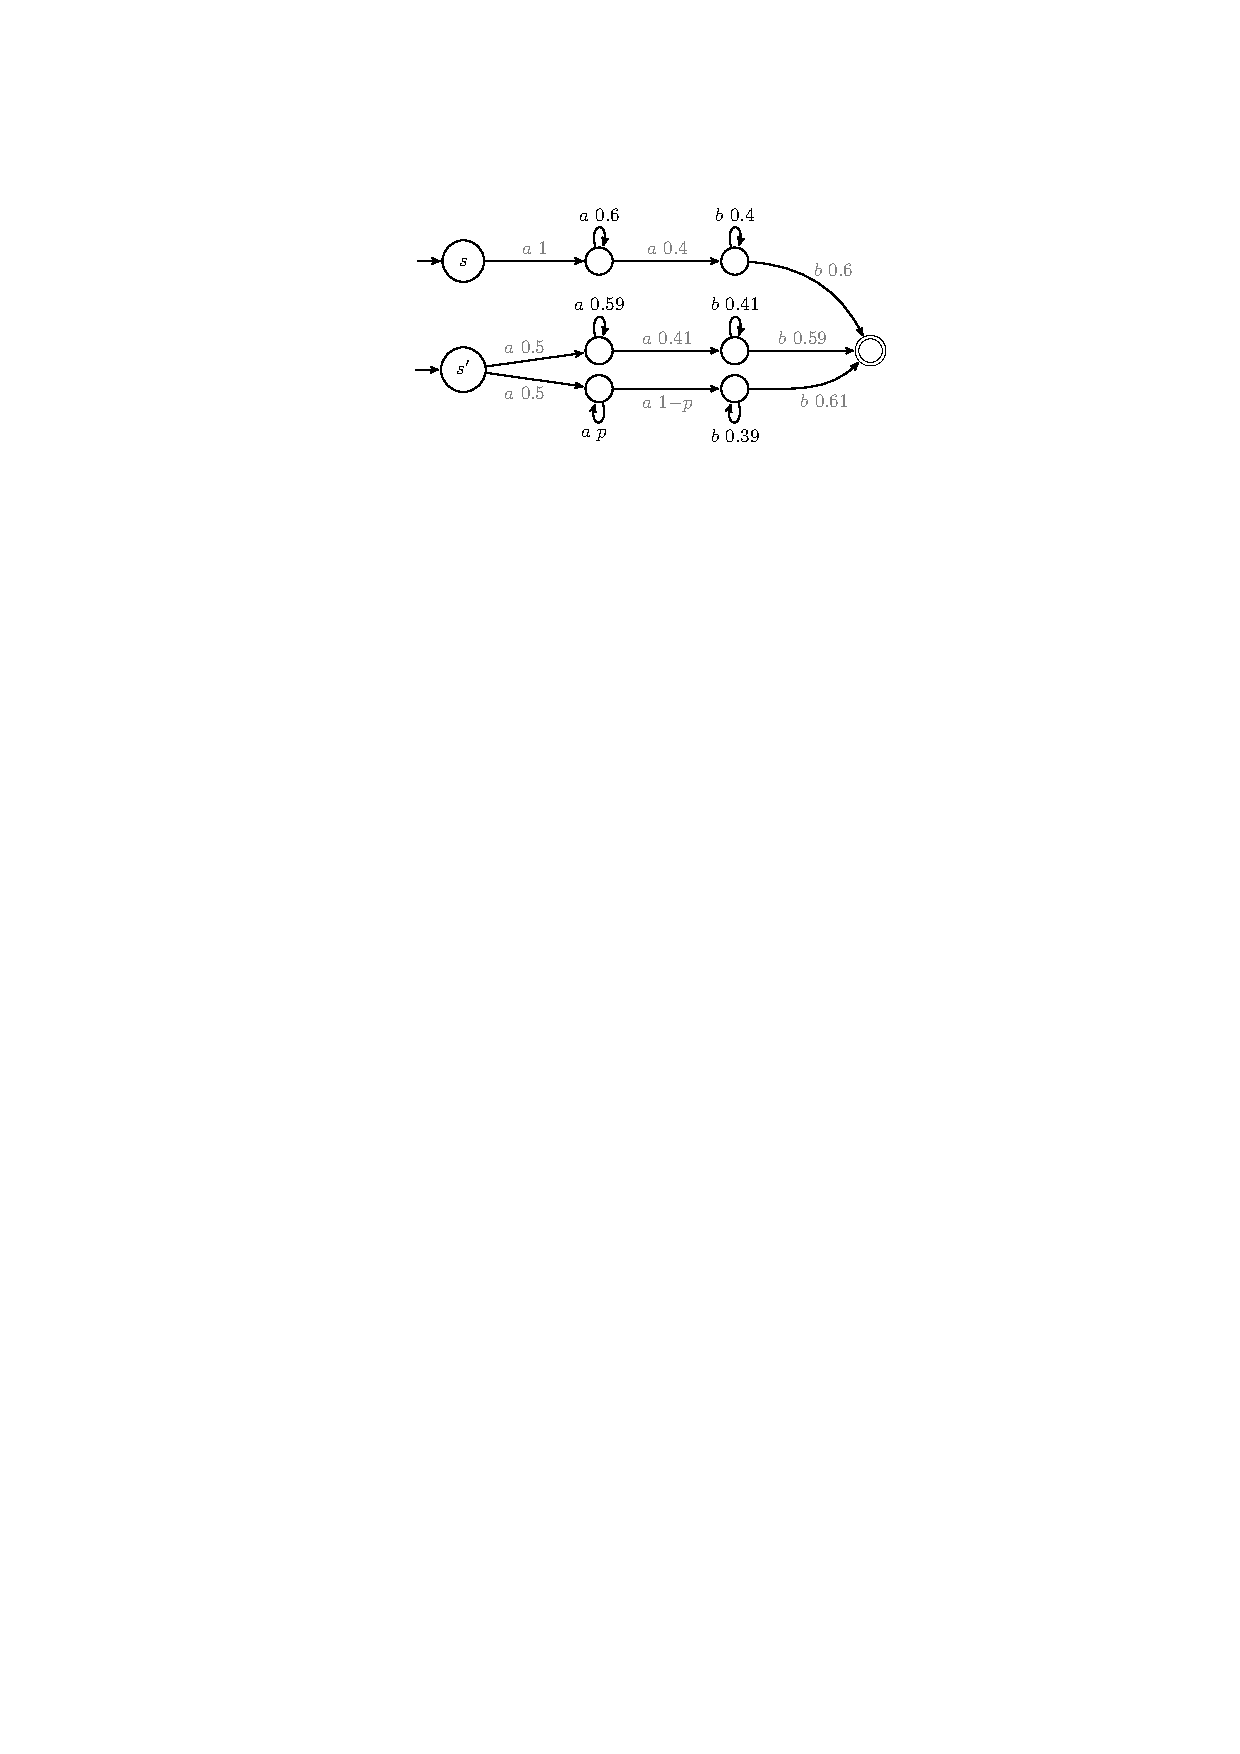
\includegraphics[width=\textwidth]{example}
            \end{figure}

        \end{column}

        \begin{column}{.42\textwidth}
            $$p \le 0.62$$
            $$\begin{cases}
                f_s(a^mb^n) & = \Theta(0.6^m0.4^n) \\
                f_{s^\prime}(a^mb^n) & = \Theta(p^m0.39^n+0.59^m0.41^n) 
            \end{cases}$$
        \end{column}
    \end{columns}
    \begin{block}{Big-O problem instance}
    When $n,m \to \infty$, does $f_s(a^mb^n) / f_{s^\prime}(a^mb^n) \to \infty$ always hold? 
    \end{block}
\end{frame}

\section{Conditional Decidability for Bounded Language}
\begin{frame}{Language Boundedness}
    Let $L \subseteq \Sigma^\prime$:

    \begin{block}{bounded \only<4->{\redbf{Conditional Decidable!}}}
        $L$ is bounded if $L \subseteq w_1^*w_2^*\cdots w_m^*$ for some $w_1,w_2,\cdots, w_m \in \Sigma^*$
        \begin{itemize}
            \item Constructed by repeating some patterns
        \end{itemize}
    \end{block}

    \only<4->{\centering \blue{$\Downarrow$ Reduce}}

    \begin{block}{letter-bounded \only<3->{\redbf{Conditional Decidable!}}}
        $L$ is letter-bounded if $L \subseteq a_1^*a_2^*\cdots a_m^*$ for some $a_1,a_2,\cdots, a_m \in \Sigma$
        \begin{itemize}
            \item Constructed by repeating some letters
        \end{itemize}
    \end{block}

    \only<3->{\centering \blue{$\Downarrow$ Reduce}}

    \begin{block}{plus-letter-bounded \only<2->{\redbf{Conditional Decidable!}}}
        $L$ is plus-letter-bounded if $L \subseteq a_1^+a_2^+\cdots a_m^+$ for some $a_1,a_2,\cdots, a_m \in \Sigma$
        \begin{itemize}
            \item Constructed by repeating certain letters $\ge 1$
        \end{itemize}
    \end{block}
\end{frame}

\begin{frame}{Conclusions}
    This paper
    \begin{itemize}
        \item keeps undecidability results of weighted automata Big-O problem in general
        \item for bounded languages,
        \begin{itemize}
            \item the result depends on a conjecture from number theory
            \item leaves open the exact borderline between decidability and undecidability
        \end{itemize}
    \end{itemize}
    Natural directions in future work
    \begin{itemize}
        \item analogous problem for infinite words
        \item further analysis on ambiguity
        \begin{itemize}
            \item e.g., is the big-O problem decidable for k-ambiguous weighted automata?
        \end{itemize}
        \item extension to negative edge weights 
    \end{itemize}
\end{frame}



\end{document}